\documentclass[12pt]{article}
\usepackage[utf8]{inputenc}
\usepackage{graphicx}
\usepackage{parskip}
\usepackage{amsfonts}
\usepackage[top=1.0in,bottom=1.0in]{geometry}


\usepackage{tikz,pgfplots}
\usetikzlibrary{calc}


\begin{document}
\pagestyle{empty}
\thispagestyle{empty}

\large
\resizebox{\linewidth}{!}{

% Sphere with great circle
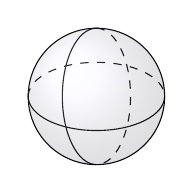
\begin{tikzpicture}[scale=\textwidth/14cm,samples=200]
    \draw (-1,0) arc (180:360:1cm and 0.5cm);
    \draw[dashed] (-1,0) arc (180:0:1cm and 0.5cm);
    \draw (0,1) arc (90:270:0.5cm and 1cm);
    \draw[dashed] (0,1) arc (90:-90:0.5cm and 1cm);
    \draw (0,0) circle (1cm);
    \shade[ball color=blue!10!white,opacity=0.20] (0,0) circle (1cm);
\end{tikzpicture}
\hspace{0.5cm}

% Mesh of gaussian
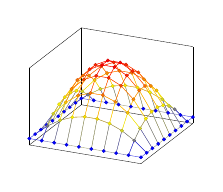
\begin{tikzpicture}[scale=\textwidth/40cm,samples=200]
    \pgfplotsset{ticks=none}
	\begin{axis}
	\addplot3+[mesh,scatter,samples=10,domain=0:1]
		{x*(1-x)*y*(1-y)};
	\end{axis}
\end{tikzpicture}

% Mobius band with center circle
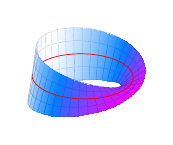
\begin{tikzpicture}[scale=\textwidth/40cm,samples=200]
  \begin{axis}[
    hide axis,
    view = {40}{40}
  ]
  \addplot3 [
    surf,
    colormap/cool,
    shader     = faceted interp,
    point meta = x,
    samples    = 40,
    samples y  = 5,
    z buffer   = sort,
    domain     = 0:360,
    y domain   =-0.5:0.5
  ] (
    {(1+0.5*y*cos(x/2)))*cos(x)},
    {(1+0.5*y*cos(x/2)))*sin(x)},
    {0.5*y*sin(x/2)}
  );

  \addplot3 [
    samples=50,
    domain=-145:180,
    samples y=0,
    thick,
    color = red
  ] (
    {cos(x)},
    {sin(x)},
    {0}
  );
  \end{axis}
\end{tikzpicture}
}

\end{document}
